\newpage
\section{Weryfikacja działania sztucznej skóry na robocie}
\label{s_testy}

Końcowym etapem projektowania rozwiązania jest użycie go w rzeczywistości i~pomyślne przejście testów działania na robocie. Zanim jednak sztuczna skóra została założona na robota została ona przetestowana w~symulatorze Gazebo. Symulator ten, opisywany szerzej w~rozdziale \ref{ss_narzedzia_gazebo}, pozwala na przetestowanie działania i~algorytmów w~bezpiecznym środowisku.

\subsection{Weryfikacja działania w symulacji}

Weryfikacja działania czujnika zaczęła się od zainstalowania całego potrzebnego oprogramowania do jego obsługi wraz z paczkami robota Tiago i środowiskiem laboratoryjnym na maszynie wirtualnej z systemem Ubuntu 18.4. Po skonfigurowaniu wszystkich portów obsługujących USB stanowisko było gotowe do testowania.

\begin{figure}[!b]
    \centering 
    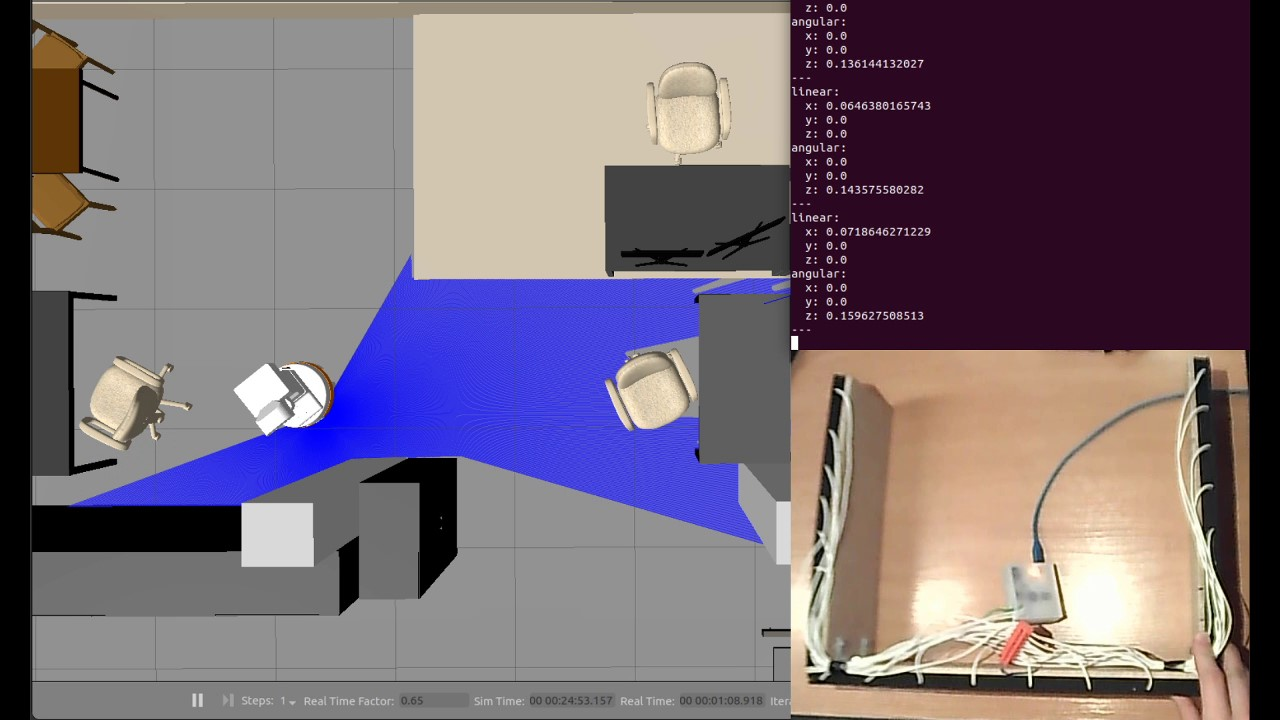
\includegraphics[width=0.95\linewidth]{img/test_gazebo.jpg}
    \caption{Test w symulatorze Gazebo wraz ze stanowiskiem i sygnałem sterującym}
    \label{f_test_gazebo}
\end{figure}

Same testy przebiegły sprawnie, wręcz bezproblemowo. Algorytm sterowania okazał się działać prawidłowo, jak również sterownik poprawnie przetwarzał i interpretował wywierany nacisk na skórę. Również część odpowiedzialna za zatrzymanie się robota przed przeszkodą prawidłowo działało. Testy w symulacji były jednak bardzo przydatne, ponieważ każda z opisanych działających funkcji została dokładniej dopracowana i dobrane zostały parametry jej działania. W sterowniku wyszła potrzeba wycięcia szumów i niskich wartości, ponieważ czujnik był niesymetryczny i sterował robotem nawet przy braku nacisku na skórę. Algorytm sterowania potrzebował dobrania poprawnych wartości wzmocnień sygnału, ponieważ te zastane nie pozwalały na płynną jazdę i obracanie się robota. Funkcja zatrzymywania się przed przeszkodą również potrzebowała lekkiego doregulowania w zakresie dystansu od przeszkody, w którym robot się zatrzymuje.

Nagranie wykonane podczas testów prezentujące jednocześnie widok symulatora Gazebo, dokładne sygnały sterujące przesyłane do robota na temacie $/key\_vel$ oraz aktualnie naciskane strefy czujnika umieszczone zostało w darmowym serwisie Vimeo \cite{b_site_vimeo_gazebo}. Screen z tego filmu został przedstawiony na rysunku \ref{f_test_gazebo}

\subsection{Weryfikacja działania na rzeczywistym robocie}

Po pomyślnej weryfikacji działania w symulacji, sztuczna skóra została zamocowana na robocie. Przejście pomiędzy tymi dwoma platformami okazało się bardzo proste. Jedyne, co było potrzebne, to podłączenie czujnika kablem USB bezpośrednio do gniazda, znajdującego się w notebooku połączonym z robotem Tiago. Po uprawnieniu do korzystania skryptu z~portu USB sztuczna skóra jest praktycznie gotowa do działania i~współpracy z~robotem.

\subsubsection{Pierwsza wersja sztucznej skóry - zakładana na tył}
Testy przeprowadzone na faktycznym robocie wykazały kilka znaczących różnic pomiędzy symulacją, a środowiskiem rzeczywistym. W trakcie testów niejednokrotnie zostały zaobserwowane zakłócenia, których nie było w symulacji. Najwieksza część wykrywanych zakłóceń pochodziła z sygnału otrzymywanego ze skanera laserowego. Otrzymywane dane posiadały czasami odczyty, które w żaden sposób nie pokrywały się ze stanem faktycznym - były całkowicie losowe. Regularnie wartości zmierzonej odległości okazywały się zbyt małe ($\sim 2mm$), aby pochodziły od jakiejkolwiek przeszkody. Pomiary te były błędnie interpretowane przez algorytm jako wykryta przeszkoda i praktycznie uniemożliwiały robotowi jakiekolwiek poruszanie się. Po odfiltrowaniu tych danych przez całkowite nieuwzględnianie ich (ponieważ są zbyt małe) zaobserwowano, że skaner laserowy ma również problem z odczytywaniem odległości w momencie kiedy w jego polu pojawiała się okrągła, metalowa noga stołu. Nie ma pewności jaka dokładnie była przyczyna tego zachowania, ale skaner laserowy czasami przesyłał mniejsze odległości, niż te występujące w~rzeczywistości. Mocno utrudniało to dojechanie do nogi stołu na odległość graniczną zapisaną w programie. W momencie, kiedy robotowi udało się dojechać do przeszkody to dalsze działania wykonywał już według ustalonego wcześniej algorytmu. Takiego zachowania nie zaobserwowano podczas testów robota na innych przeszkodach jak ściana czy krzesła.

Ważne było także ciągłe uważanie na zachowanie robota, czy samoczynnie nie wykonuje niepożądanych lub niebezpiecznych ruchów. Podczas wykonywanych prac nie zaobserwowano takich zachowań, ale w razie ich wystąpienia cały czas była osoba gotowa do naciśnięcia przycisku awaryjnego, znajdującego się u podstawy robota. Ewentualne nieopanowanie robota wiązałoby się z potencjalnie sporymi stratami materialnymi. Dlatego też użyte algorytmy zostały wcześniej pomyślnie przetestowane w symulacji. Robot w trakcie testów został przedstawiony na rysunku \ref{f_test_robot_1}.

\begin{figure}[!h]
    \centering 
    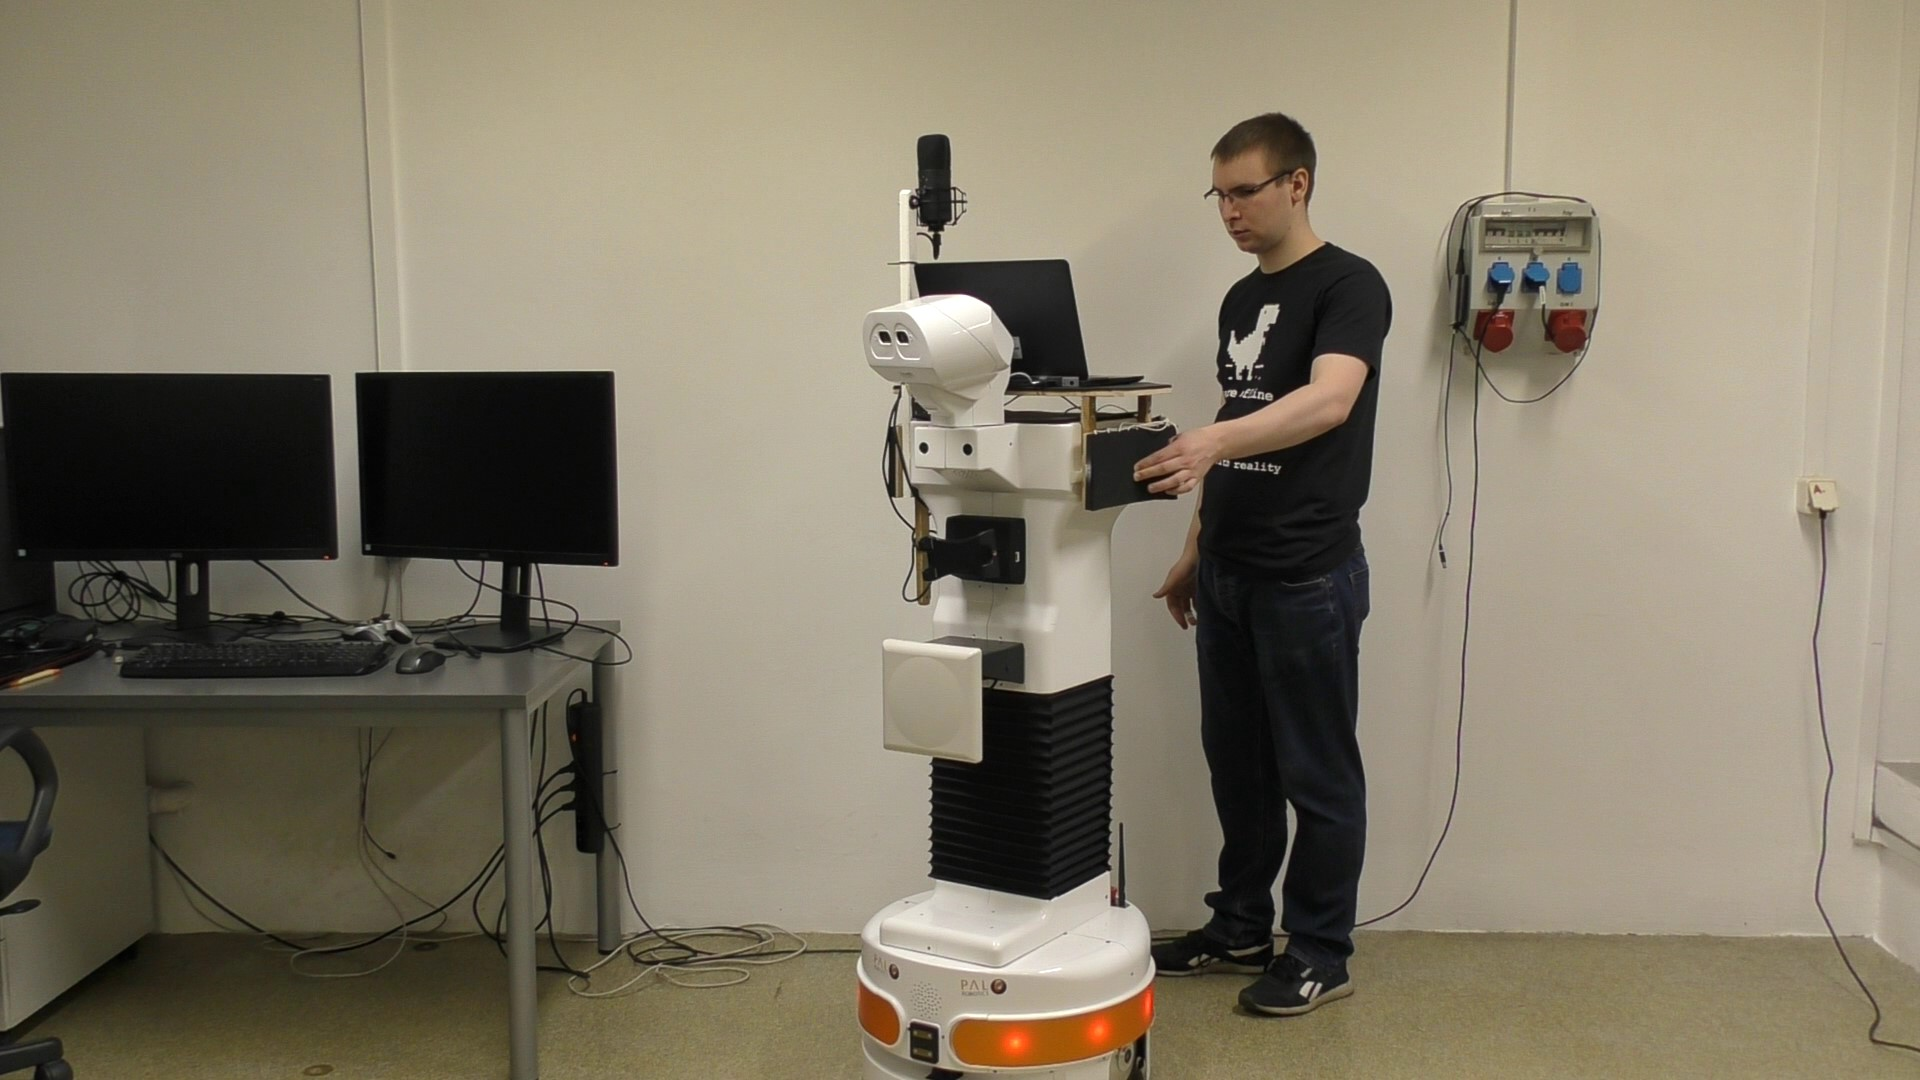
\includegraphics[width=0.95\linewidth]{img/test_robot_1.jpg}
    \caption{Robot Tiago podczas testów}
    \label{f_test_robot_1}
\end{figure}

Podczas użytkowania i sprawdzania poprawności zaimplementowanych rozwiązań wzięto pod uwagę kilka dodatkowych nieznacznych poprawek. Poza zaszumionym sygnałem otrzymywanym ze skanera laserowego okazało się także, że nie ma on zasięgu $\ang{220}$, jak~w~symulatorze, tylko $\ang{190}$ ($\pm\ang{95}$). Zostały także ustawione inne dopuszczalne odległości robota do przedmiotów. Wartość ta została zmniejszona z $40cm$ do $30cm$. Poza tymi małymi poprawkami kod przeniesiony z symulatora od razu nadawał się do korzystania z~robota.

Podczas używania prototypu wykonano kilka podstawowych testów jego działania. Pierwszy i podstawowy test polegał na sterowaniu robotem za pomocą naciskania na różne obszary sztucznej skóry. Test ten został wykonany pomyślnie i bez większych problemów. Został także wykonany, opisywany już wcześniej, test współpracy ze skanerem laserowym, gdzie sam program działał dobrze, lecz czujnik odległości czasami wysyłał błędne dane. Zostały też wykonane testy zachowania robota na uderzenia i statyczny nacisk. Test~działania na uderzenie przebiegł całkiem pomyślnie. Należy jednak zauważyć, że~to~czujnik przyjął większą część siły uderzenia, a sam robot odjechał dopiero po chwili. Testy~wykonane na statycznym nacisku (przedmiotem, który nie zmienia swojego położenia w czasie) pokazały niestety sporą wadę wykonanego czujnika - jego kształt. Zaprojektowany kształt posiadający kąty ostre powodował, że~w~pierwszej fazie, przy próbie obrotu robot mocniej naciskał na statyczny przedmiot, a nie jak zakładano zmniejszał ten nacisk. Jest to ogólny problem mocno związany z~napędem różnicowym robota, który przed jazdą w przód musi się najpierw cały obrócić. Nagranie z~wykonanych na robocie testów dostępne jest na serwisie Vimeo \cite{b_site_vimeo_kwadrat}.

\subsubsection{Finalna wersja sztucznej skóry - dookolna}

Testy wykonane na pierwszej wersji sztucznej skóry, wykazały jeden kluczowy błąd, który wynikał z użytego kształtu szkieletu. Niestety ta wada powodowała, że rozwiązanie nie spełniało jednego z głównych założeń sztucznej skóry - nie wywierania siły na środowisko. W momencie wykrywania nacisku z boku i obracania się w miejscu, robot wywoływał jeszcze większy nacisk na środowisko. Było to powodem budowy drugiej wersji sztucznej skóry opartej na okrągłym szkielecie, który pozbawiony jest tej wady.

Cała konstrukcja, poza częścią mechaniczną, pozostała dokładnie taka sama. Kolejne warstwy sztucznej skóry również zostały złożone w tej samej kolejności. Zmodyfikowana została tylko konfiguracja pól czujnika. 

Do budowy szkieletu wykorzystana została obręcz rowerowa $26" (1.5/559)$ o szerokości $2.5 cm$. Zewnętrzna część tej obręczy ma minimalnie większy obwód niż dolny obwód robota Tiago, dzięki czemu wykonany na nim czujnik nie zwiększy znacząco całkowitego promienia, który robot zajmuje w środowisku. Na zewnętrznej części obręczy zamocowana została za pomocą nitów blacha ocynkowana $0.5 mm$ o szerokości $120 mm$. Blacha ta zapewnia odpowiedni kompromis pomiędzy sztywnością konstrukcji, a pochłanianiem siły uderzeń. Do blachy zostały przyklejone taśmą montażową kolejne warstwy sztucznej skóry w sposób identyczny, jak opisany w rozdziale \ref{ss_integracja_budowa}.
Zbudowany szkielet został zamocowany do robota Tiago za pomocą lekkich listew drewnianych, śrub i wkrętów. 
Wykonanie takiej konstrukcji w pełni spełnia wymagania warstwy mechanicznej opisanej w rozdziale \ref{ss_budowa_mech}. Postępy prac nad budową drugiej wersji prototypu zostały przedstawione na rysunku \ref{f_test_prace_1}, a~zbudowany prototyp na rysunku \ref{f_test_ready_1}. Prototyp ten składa się z~$32$~pól sensorycznych, które są równomiernie rozłożone na całym okręgu, z~dodaniem $8$~pól, na~których nie ma umieszczonego czujnika. 
Obecność kilku pól bez czujnika wynika z~faktu, że~nie mógł on zostać tam zamocowany z~powodu łączenia się poziomych odcinków folii miedzianej oraz fizycznych ograniczeń sterownika. Wspomniana nowa konfiguracja sztucznej skóry została przedstawiona w~tabeli \ref{t_test_2_config}.

\begin{figure}[!h]
    \centering 
    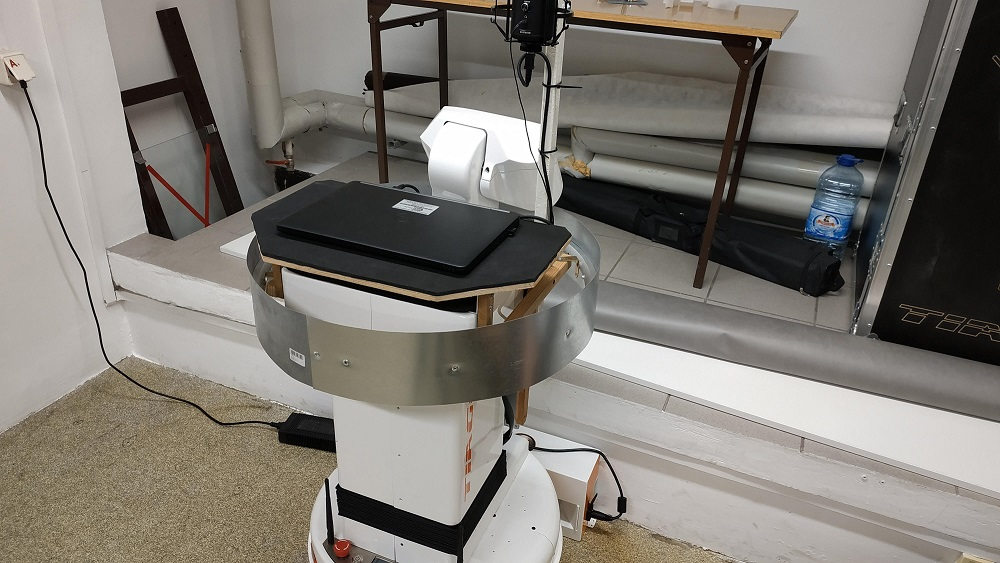
\includegraphics[width=0.95\linewidth]{img/test_okr_prace_1.jpg}
    \caption{Postęp prac prowadzonych nad drugim prototypem sztucznej skóry}
    \label{f_test_prace_1}
\end{figure}

\begin{table}[!h]
\centering
\caption{Konfiguracja pól czujnika drugiej wersji sztucznej skóry}
\begin{tabular}{|l|l|rrrr|}
\hline
\rowcolor[HTML]{FFFFFF} 
 &
   &
  \multicolumn{1}{l|}{\cellcolor[HTML]{FFFFFF}Kolumna 1} &
  \multicolumn{1}{l|}{\cellcolor[HTML]{FFFFFF}Kolumna 2} &
  \multicolumn{1}{l|}{\cellcolor[HTML]{FFFFFF}Kolumna 3} &
  \multicolumn{1}{l|}{\cellcolor[HTML]{FFFFFF}Kolumna 4} \\ \hline
\rowcolor[HTML]{C0C0C0} 
\cellcolor[HTML]{FFFFFF}                         & Kąt       & 0° &90° & 180°  & 270°  \\ \cline{2-2}
\rowcolor[HTML]{EFEFEF} 
\multirow{-2}{*}{\cellcolor[HTML]{FFFFFF}Rząd 1} & Odległość & 1    & 1    & 1    & 1     \\ \cline{1-2}
\rowcolor[HTML]{C0C0C0} 
\cellcolor[HTML]{FFFFFF}                         & Kąt       & 9° & 99° & 189°  & 279°  \\ \cline{2-2}
\rowcolor[HTML]{EFEFEF} 
\multirow{-2}{*}{\cellcolor[HTML]{FFFFFF}Rząd 2} & Odległość & 1    & 1    & 1    & 1   \\ \cline{1-2}
\rowcolor[HTML]{C0C0C0} 
\cellcolor[HTML]{FFFFFF}                         & Kąt       & 18° & 108° & 198°  & 288°  \\ \cline{2-2}
\rowcolor[HTML]{EFEFEF} 
\multirow{-2}{*}{\cellcolor[HTML]{FFFFFF}Rząd 3} & Odległość & 1    & 1    & 1    & 1     \\ \cline{1-2}
\rowcolor[HTML]{C0C0C0} 
\cellcolor[HTML]{FFFFFF}                         & Kąt       & 27° & 117° & 207°  & 297° \\ \cline{2-2}
\rowcolor[HTML]{EFEFEF} 
\multirow{-2}{*}{\cellcolor[HTML]{FFFFFF}Rząd 4} & Odległość & 1    & 1    &1    & 1    \\ \cline{1-2}
\rowcolor[HTML]{C0C0C0} 
\cellcolor[HTML]{FFFFFF}                         & Kąt       & 45° & 135° & 225° & 315°\\ \cline{2-2}
\rowcolor[HTML]{EFEFEF} 
\multirow{-2}{*}{\cellcolor[HTML]{FFFFFF}Rząd 5} & Odległość & 1    & 1    & 1    & 1     \\ \cline{1-2}
\rowcolor[HTML]{C0C0C0} 
\cellcolor[HTML]{FFFFFF}                         & Kąt       & 54° & 144° & 234°  & 324°  \\ \cline{2-2}
\rowcolor[HTML]{EFEFEF} 
\multirow{-2}{*}{\cellcolor[HTML]{FFFFFF}Rząd 6} & Odległość & 1    & 1    & 1    & 1     \\ \cline{1-2}
\rowcolor[HTML]{C0C0C0} 
\cellcolor[HTML]{FFFFFF}                         & Kąt       & 63° & 153° & 243° & 333° \\ \cline{2-2}
\rowcolor[HTML]{EFEFEF} 
\multirow{-2}{*}{\cellcolor[HTML]{FFFFFF}Rząd 7} & Odległość & 1    & 1    & 1    & 1     \\ \cline{1-2}
\rowcolor[HTML]{C0C0C0} 
\cellcolor[HTML]{FFFFFF}                         & Kąt       & 72° & 162° & 252°  & 342°  \\ \cline{2-2}
\rowcolor[HTML]{EFEFEF} 
\multirow{-2}{*}{\cellcolor[HTML]{FFFFFF}Rząd 8} & Odległość & 1    & 1    & 1    & 1     \\ \cline{1-2}
\hline
\end{tabular}
\label{t_test_2_config}
\end{table}

Zbudowana sztuczna skóra od razu po okablowaniu i~wgraniu nowej konfiguracji była gotowa do działania. Z~uwagi na to, że algorytm sterowania został wcześniej przetestowany na robocie i~działał poprawnie, zrezygnowano z~testów drugiego prototypu w symulatorze Gazebo i~od razu przystąpiono do testów na robocie. Algorytm pomimo już poprawnego wcześniej działania został dodatkowo usprawniony poprzez dodanie do niego dobranej doświadczalnie rampy na sterowaniu prędkością, zarówno jazdy, jak i~obracania się. Rampa~ta została zaimplementowana w~celu złagodzenia bardzo gwałtownych skoków robota spowodowanych wykryciem nacisku na sztuczną skórę, widocznych wyraźnie podczas poprzednich testów. Minusem takiego podejścia jest wyraźne zwiększenie się czasu, jaki~Tiago potrzebuje, aby~odjechać od źródła kolizji.

\begin{figure}[!h]
    \centering 
    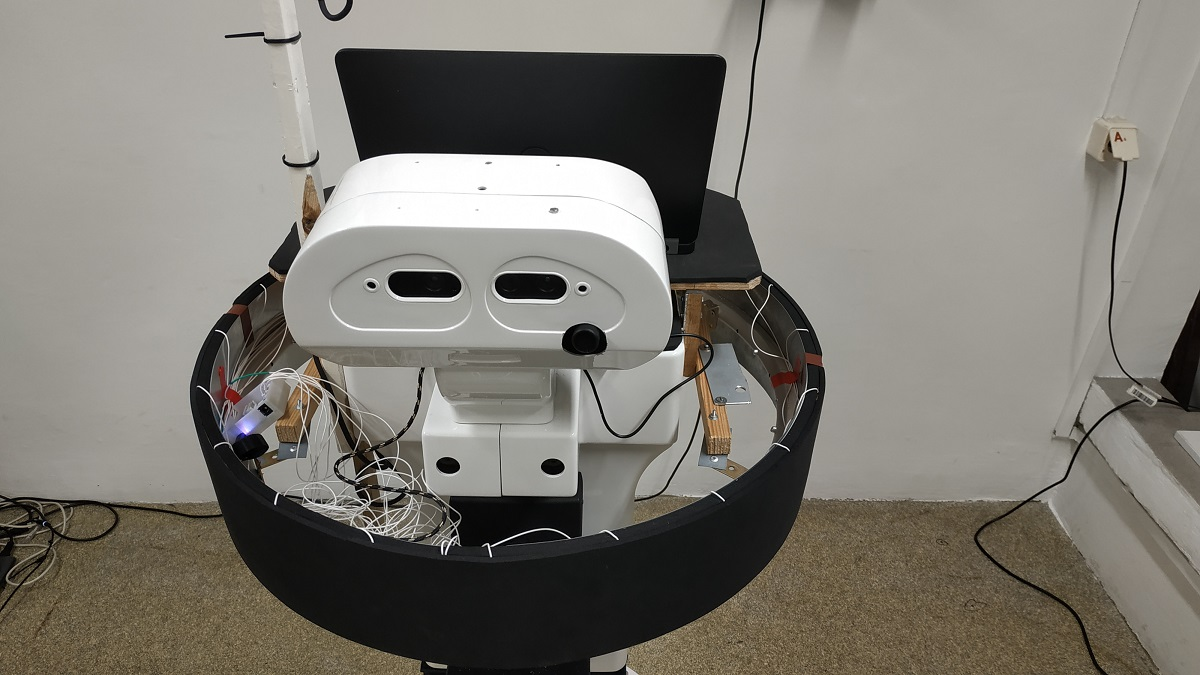
\includegraphics[width=0.95\linewidth]{img/test_okr_ready_2.jpg}
    \caption{Druga wersja prototypowej sztucznej skóry}
    \label{f_test_ready_1}
\end{figure}

Przeprowadzone testy obejmowały podobny zakres co testy pierwszego prototypu. Pierwszy test polegał na teście pracy i zachowania robota pod wpływem generowania nacisku na różnych częściach sztucznej skóry. Test przebiegł pozytywnie, a odczucia były lepsze niż w przypadku pierwszego prototypu. Zachowanie robota wydawało się lepiej odzwierciedlać miejsce, w którym robot był naciskany. Szczególnie mocno zauważalne było użycie rampy na sygnale sterującym, które spowodowało widoczne upłynnienie ruchów robota i zniwelowanie wykonywanych przez niego wcześniej szarpnięć. Dzięki nowej konstrukcji zaistniała także możliwość przetestowania reakcji Tiago na nacisk z~przodu robota, czego nie dało się wykonać w poprzedniej konstrukcji. Kolejnym testem był test współpracy sztucznej skóry z czujnikiem odległości. Przyniósł on tak samo dobre wyniki jak poprzednia iteracja sensora. 

Ostatnim z testów było przyłożenie robota nacisku, który nie zmienia swojej pozycji w~przestrzeni. Test ten przebiegł dużo pozytywniej niż w poprzedniej wersji czujnika. Czas odjazdu się co prawda wydłużył, ale~sam ruch robota był dużo płynniejszy. Okrągła wersja czujnika została prawidłowo umieszczona w~centrum osi obrotu robota, dzięki czemu w~przypadku nacisku na którykolwiek z~kierunków robot nie generował zwiększającego się nacisku na otoczenie. Działający robot w trakcie testów został przedstawiony na rysunku~\ref{f_test_test_1}.

%Nagranie z testów zostało udostępnione także na serwisie Vimeo https://vimeo.com/manage/videos/553825354

\begin{figure}[!h]
    \centering 
    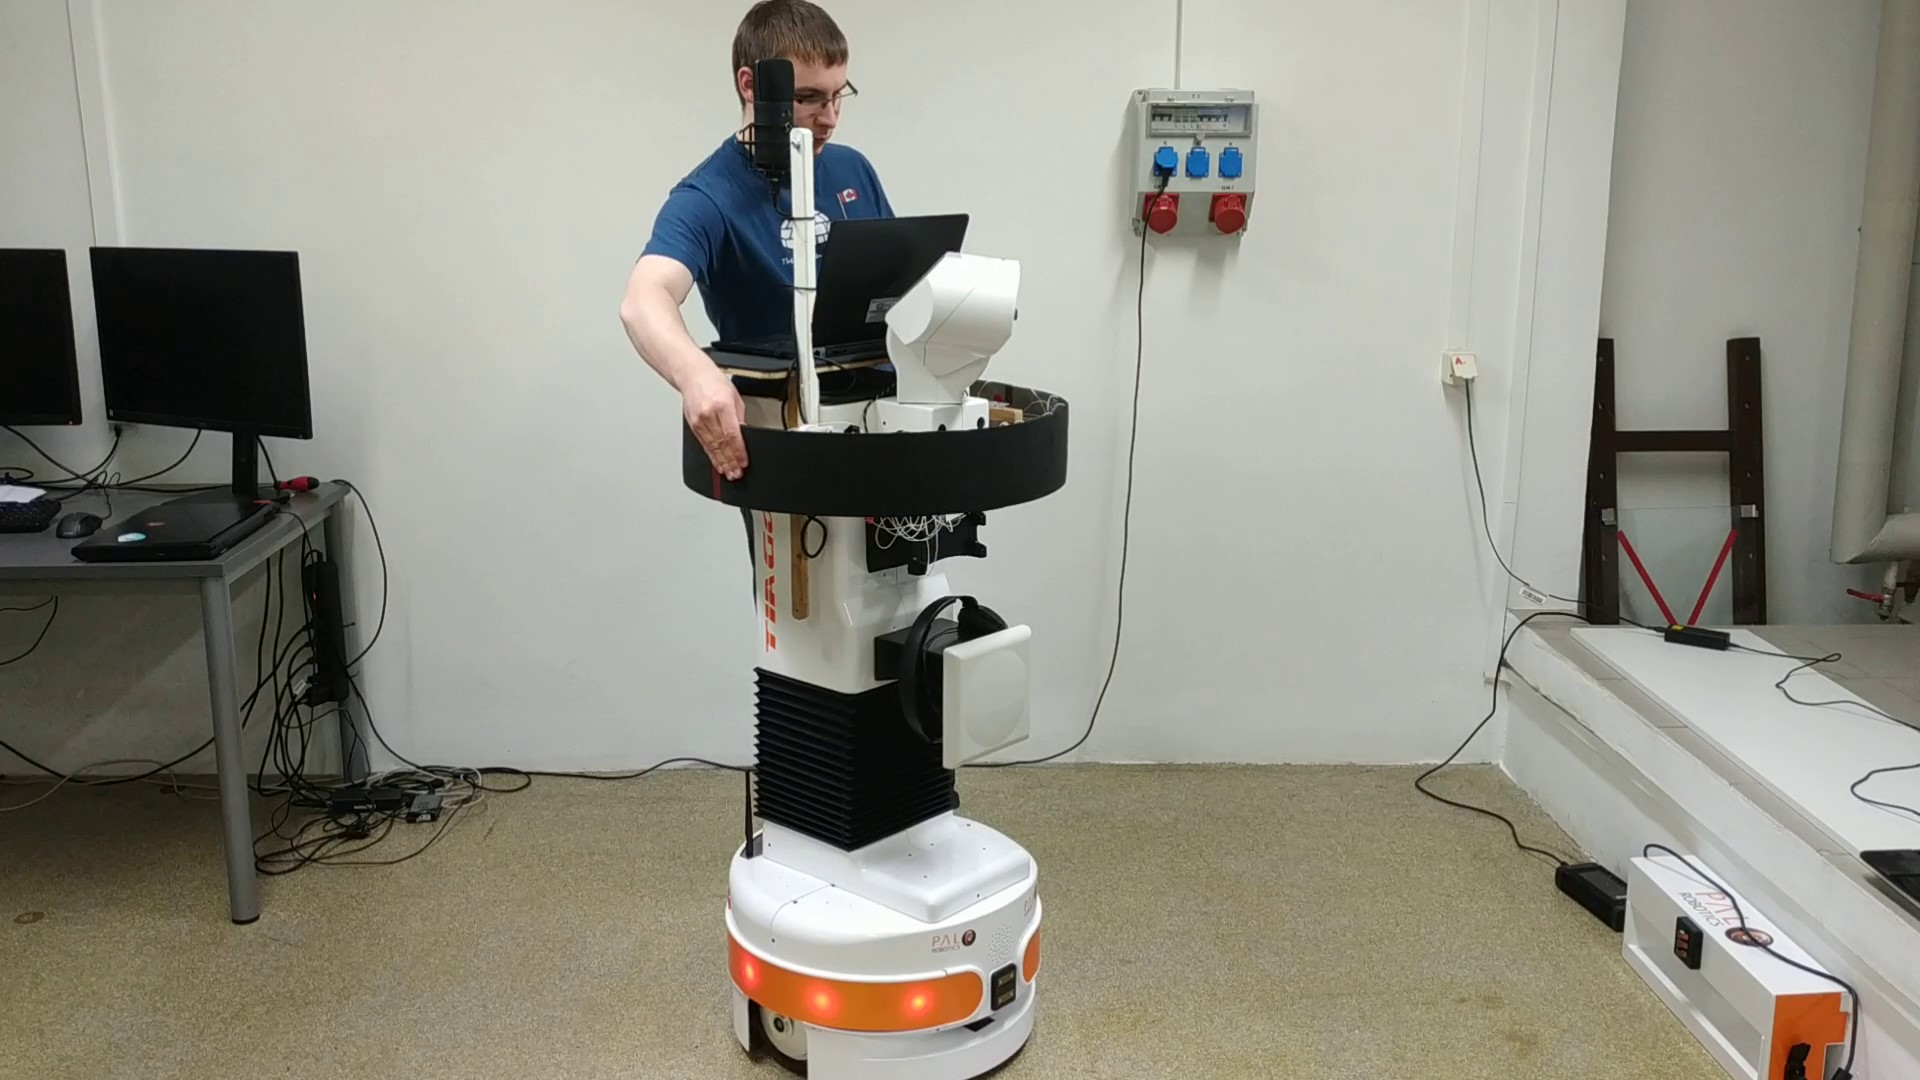
\includegraphics[width=0.95\linewidth]{img/test_okr_test_1.jpg}
    \caption{Druga wersja prototypowej sztucznej skóry podczas testów na robocie}
    \label{f_test_test_1}
\end{figure}

Podczas praktycznych testów Tiago wraz z jego pozostałymi podzespołami pojawiły się kolejne elementy, które musiały zostać poprawione. Krytycznym błędem okazał się fakt, że~zamocowana na robocie sztuczna skóra w sposób znaczący ogranicza jego pole widzenia. Było to na tyle znaczące uchybienie, że~wymogło ono znaczącą zmianę miejsca mocowania sztucznej skóry. Finalnie, została ona zamocowana u podstawy robota, zaraz nad czujnikami odległości. Takie miejsce mocowania jest sprzeczne z~postawionymi na początku pracy założeniami, lecz jest to rozbieżność konieczna do zaakceptowania, aby~można było uznać czujnik za poprawnie zintegrowany z robotem. Zdjęcie nowego zamocowania czujnika skóry zostało przedstawione na rysunku \ref{f_test_test_2}.

\begin{figure}[!h]
    \centering 
    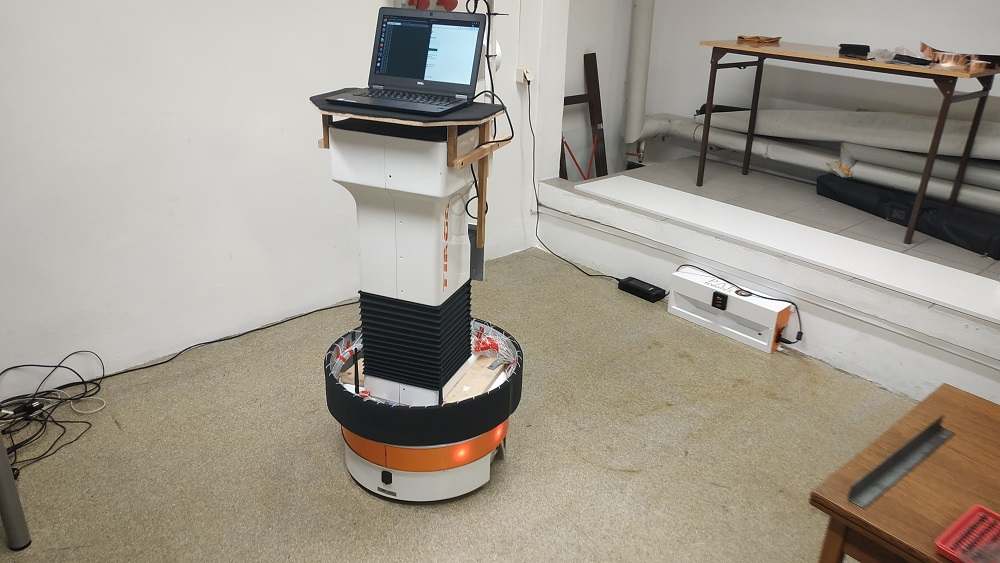
\includegraphics[width=0.95\linewidth]{img/test_okr_test_2.jpg}
    \caption{Druga wersja prototypowej sztucznej skóry zamocowana u podstawy robota}
    \label{f_test_test_2}
\end{figure}

W trakcie integracji sztucznej skóry z pozostałymi modułami robota wynikł także błąd powodujący problemy z automatyczną nawigacją robota, która przestała działać. Wynikał on z faktu, że robot wysyłał swoje żądania zadające prędkość na priorytecie wyższym niż te wysyłane przez moduł nawigacji. W ten sposób moduł sztucznej skóry po pierwszym wysłaniu żądania blokował kanał sterowania prędkością w taki sposób, że niemożliwa była jego dezaktywacja. Jedynym sposobem na ponowne odblokowanie kanału sterowania było w~takim przypadku ponowne uruchomienie całego robota. Jest to jednak zbyt drastyczne i~niepraktyczne podejście. Aby umożliwić zdalne dezaktywowanie sygnałów wysyłanych przez sztuczną skórę, węzeł w systemie ROS obsługujący sztuczną skórę, poza wykonywanymi wcześniej czynnościami nasłuchuje także na temacie $/artificial\_skin/reset$, czy powinien zresetować stan sztucznej skóry. Po otrzymaniu sygnału na tym temacie węzeł zaprzestaje dalszego wysyłania żądań prędkości. Węzeł sztucznej skóry dodatkowo publikuje także informację o~tym, czy sztuczna skóra została aktywowana (i wysyła żądania prędkości), tak aby inne węzły wiedziały, czy przed wysłaniem swoich żądań nie należy dezaktywować sztucznej skóry. Temat, na~którym węzeł wysyła informacje o aktywacji to:~$/artificial\_skin/activated$. Nowy schemat behawioralny, uwzględniający naniesione w końcowej fazie projektu poprawki, węzła sztucznej skóry robota został przedstawiony na rysunku \ref{f_behaw}.

\begin{figure}[!h]
    \centering 
    \includegraphics[width=0.95\linewidth]{img/behawioral.pdf}
    \caption{Schemat behawioralny węzła sztucznej skóry w systemie ROS}
    \label{f_behaw}
\end{figure}

Ostatecznie, zostały przeprowadzone jeszcze jedne testy ze sztuczną skórą zamocowaną u podstawy robota i wprowadzonymi korektami w skrypcie sterującym. Testy miały identyczny charakter jak te przeprowadzane wcześniej. Nowootrzymane wyniki testów zgadzały się z tymi, które zostały uzyskane na tej samej skórze zamocowanej w górnej części robota, co dodatkowo dowodzi o skuteczności i poprawności działania modułu. Nagranie z testów zostało udostępnione także, jak poprzednie nagrania, na serwisie Vimeo \cite{b_site_vimeo_okrag}.

Druga wersja sztucznej skóry okazuje się być bardzo dobra i dobrze radzi sobie z~ochroną robota przed potencjalnymi kolizjami. Jest jednocześnie delikatna, jak również potrafi zabsorbować większe uderzenia. Liczba zamocowanych pól w zupełności wystarcza do sprawnego sterowania robotem, a samo sterowanie jazdą robota okazuje się być bardzo płynne. Finalna wersja prototypu sztucznej skóry jest też bardzo czuła, a~do~sterowania robotem za jej pomocą nie potrzeba dużej ilości siły.
